\documentclass[tikz,border=8pt]{standalone}
\usepackage{tikz}
\usepackage{amsmath,amssymb}
\usetikzlibrary{arrows.meta,positioning,calc}

\begin{document}
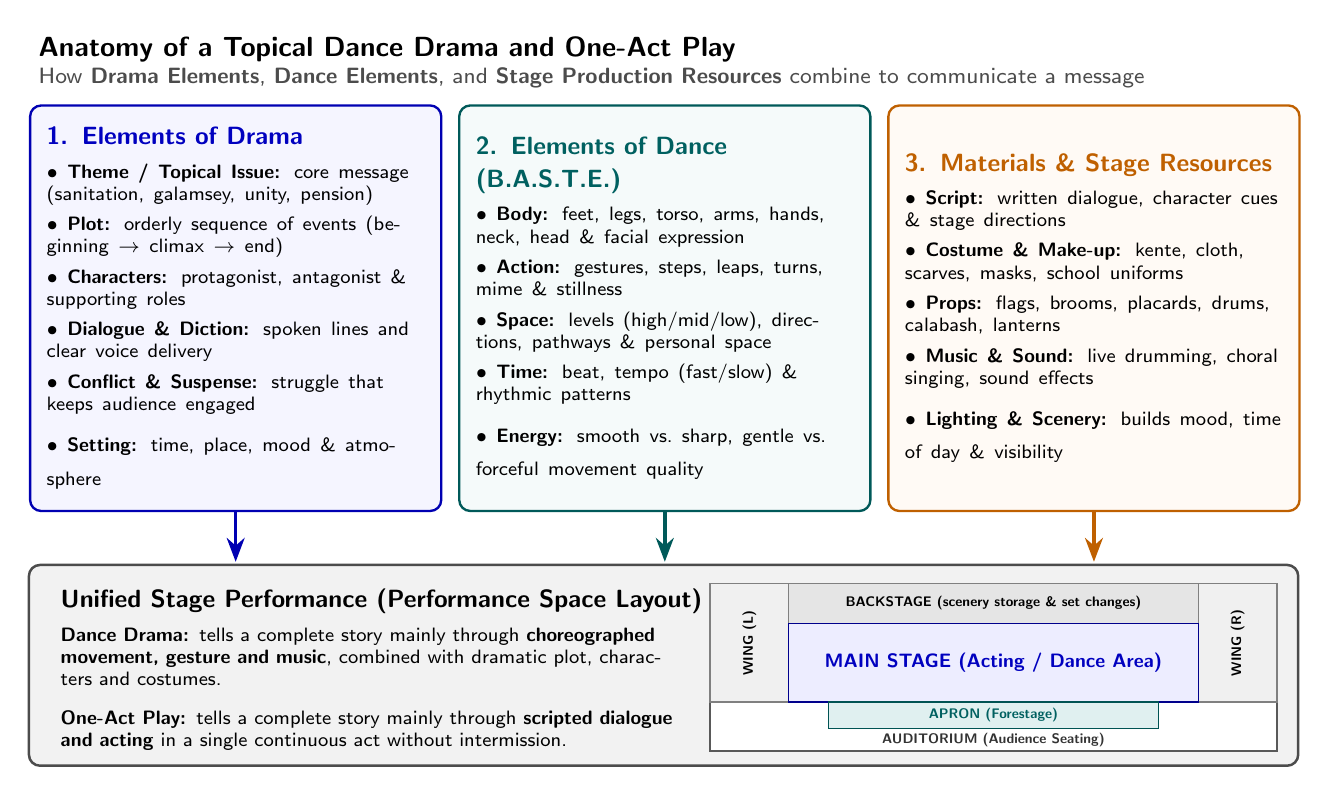
\begin{tikzpicture}[
    font=\sffamily,
    >=Stealth,
    card/.style={
        rounded corners=4pt,
        line width=0.85pt,
        inner sep=6pt,
        text width=4.80cm,
        minimum height=5.15cm,
        align=left
    }
]

% Title (y = 9.15, subtitle = 8.78)
\node[font=\sffamily\bfseries\normalsize, anchor=west] at (0, 9.15)
    {Anatomy of a Topical Dance Drama and One-Act Play};
\node[font=\sffamily\footnotesize, text=black!70, anchor=west] at (0, 8.78)
    {How \textbf{Drama Elements}, \textbf{Dance Elements}, and \textbf{Stage Production Resources} combine to communicate a message};

% Three equal-height cards anchored at north west (y = 8.45 down to y = 3.30)
\node[card, draw=blue!70!black, fill=blue!4, anchor=north west] (drama) at (0, 8.45) {
    {\bfseries\small\color{blue!75!black}1. Elements of Drama}\\[4pt]
    \scriptsize
    $\bullet$ \textbf{Theme / Topical Issue:} core message (sanitation, galamsey, unity, pension)\\[3pt]
    $\bullet$ \textbf{Plot:} orderly sequence of events (beginning $\to$ climax $\to$ end)\\[3pt]
    $\bullet$ \textbf{Characters:} protagonist, antagonist \& supporting roles\\[3pt]
    $\bullet$ \textbf{Dialogue \& Diction:} spoken lines and clear voice delivery\\[3pt]
    $\bullet$ \textbf{Conflict \& Suspense:} struggle that keeps audience engaged\\[3pt]
    $\bullet$ \textbf{Setting:} time, place, mood \& atmosphere
};

\node[card, draw=teal!70!black, fill=teal!4, anchor=north west] (dance) at (5.45, 8.45) {
    {\bfseries\small\color{teal!75!black}2. Elements of Dance (B.A.S.T.E.)}\\[4pt]
    \scriptsize
    $\bullet$ \textbf{Body:} feet, legs, torso, arms, hands, neck, head \& facial expression\\[3pt]
    $\bullet$ \textbf{Action:} gestures, steps, leaps, turns, mime \& stillness\\[3pt]
    $\bullet$ \textbf{Space:} levels (high/mid/low), directions, pathways \& personal space\\[3pt]
    $\bullet$ \textbf{Time:} beat, tempo (fast/slow) \& rhythmic patterns\\[3pt]
    $\bullet$ \textbf{Energy:} smooth vs.\ sharp, gentle vs.\ forceful movement quality
};

\node[card, draw=orange!75!black, fill=orange!4, anchor=north west] (prod) at (10.90, 8.45) {
    {\bfseries\small\color{orange!75!black}3. Materials \& Stage Resources}\\[4pt]
    \scriptsize
    $\bullet$ \textbf{Script:} written dialogue, character cues \& stage directions\\[3pt]
    $\bullet$ \textbf{Costume \& Make-up:} kente, cloth, scarves, masks, school uniforms\\[3pt]
    $\bullet$ \textbf{Props:} flags, brooms, placards, drums, calabash, lanterns\\[3pt]
    $\bullet$ \textbf{Music \& Sound:} live drumming, choral singing, sound effects\\[3pt]
    $\bullet$ \textbf{Lighting \& Scenery:} builds mood, time of day \& visibility
};

% Clean downward arrows from card bottoms (y=3.30) to banner top (y=2.62)
\draw[->, line width=1.25pt, blue!70!black] (drama.south) -- (drama.south |- 0,2.64);
\draw[->, line width=1.25pt, teal!70!black] (dance.south) -- (dance.south |- 0,2.64);
\draw[->, line width=1.25pt, orange!75!black] (prod.south) -- (prod.south |- 0,2.64);

% Bottom Fusion Banner (y = 0.05 .. 2.60) — cleanly below all cards!
\draw[rounded corners=4pt, draw=black!70, fill=black!5, line width=0.9pt] (0, 0.05) rectangle (16.12, 2.60);

% Left side of banner: title and two clean paragraphs
\node[font=\sffamily\bfseries\small, anchor=north west] at (0.28, 2.42)
    {Unified Stage Performance (Performance Space Layout)};
\node[font=\sffamily\scriptsize, anchor=north west, text width=7.90cm] at (0.28, 1.92) {
    \textbf{Dance Drama:} tells a complete story mainly through \textbf{choreographed movement, gesture and music}, combined with dramatic plot, characters and costumes.\\[6pt]
    \textbf{One-Act Play:} tells a complete story mainly through \textbf{scripted dialogue and acting} in a single continuous act without intermission.
};

% Right side of banner: Mini Performance Space Plan
\begin{scope}[shift={(8.65, 0.24)}]
    \draw[fill=white, draw=black!65, line width=0.75pt] (0, 0) rectangle (7.20, 2.12);
    % Backstage
    \draw[fill=black!10, draw=black!50] (1.00, 1.62) rectangle (6.20, 2.12);
    \node[font=\sffamily\tiny\bfseries] at (3.60, 1.87) {BACKSTAGE (scenery storage \& set changes)};
    % Wings
    \draw[fill=black!6, draw=black!50] (0, 0.62) rectangle (1.00, 2.12);
    \node[font=\sffamily\tiny\bfseries, rotate=90] at (0.50, 1.37) {WING (L)};
    \draw[fill=black!6, draw=black!50] (6.20, 0.62) rectangle (7.20, 2.12);
    \node[font=\sffamily\tiny\bfseries, rotate=90] at (6.70, 1.37) {WING (R)};
    % Main stage
    \draw[fill=blue!7, draw=blue!55!black] (1.00, 0.62) rectangle (6.20, 1.62);
    \node[font=\sffamily\scriptsize\bfseries, text=blue!75!black] at (3.60, 1.12) {MAIN STAGE (Acting / Dance Area)};
    % Apron
    \draw[fill=teal!12, draw=teal!65!black] (1.50, 0.28) rectangle (5.70, 0.62);
    \node[font=\sffamily\tiny\bfseries, text=teal!75!black] at (3.60, 0.45) {APRON (Forestage)};
    % Auditorium
    \node[font=\sffamily\tiny\bfseries, text=black!80] at (3.60, 0.14) {AUDITORIUM (Audience Seating)};
\end{scope}

\end{tikzpicture}
\end{document}
